\chapter{Gestión de Usuarios y Acceso}

\section{Registro e Inicio de Sesión}

Para comenzar a utilizar las funcionalidades de \textit{MDAA}, es necesario disponer de una cuenta de usuario. La aplicación gestiona la autenticación de manera segura, permitiendo registrar nuevos usuarios e iniciar sesión a aquellos que ya poseen credenciales.

\begin{figure}[!ht]
    \centering
    
\includegraphics[width=0.5\textwidth]{imagenes/02_usuario/01_botoneraLoginORegistro.png}
    \caption{Botonera de acceso y registro en la barra superior.}
\end{figure}

En la parte superior derecha de la pantalla de inicio, se encuentran las opciones de acceso. El usuario puede:
\begin{itemize}
    \item \textbf{Iniciar Sesión:} Si ya dispone de una cuenta verificada.
    \item \textbf{Registrarse:} Para crear una nueva cuenta y poder acceder a la creación de proyectos.
\end{itemize}

\subsection{Creación de un Nuevo Usuario}

Al seleccionar la opción de registro, se presenta un formulario de creación de cuenta. Es vital proporcionar datos precisos, especialmente el correo electrónico, ya que se requerirá su verificación.

\begin{figure}[!ht]
    \centering
    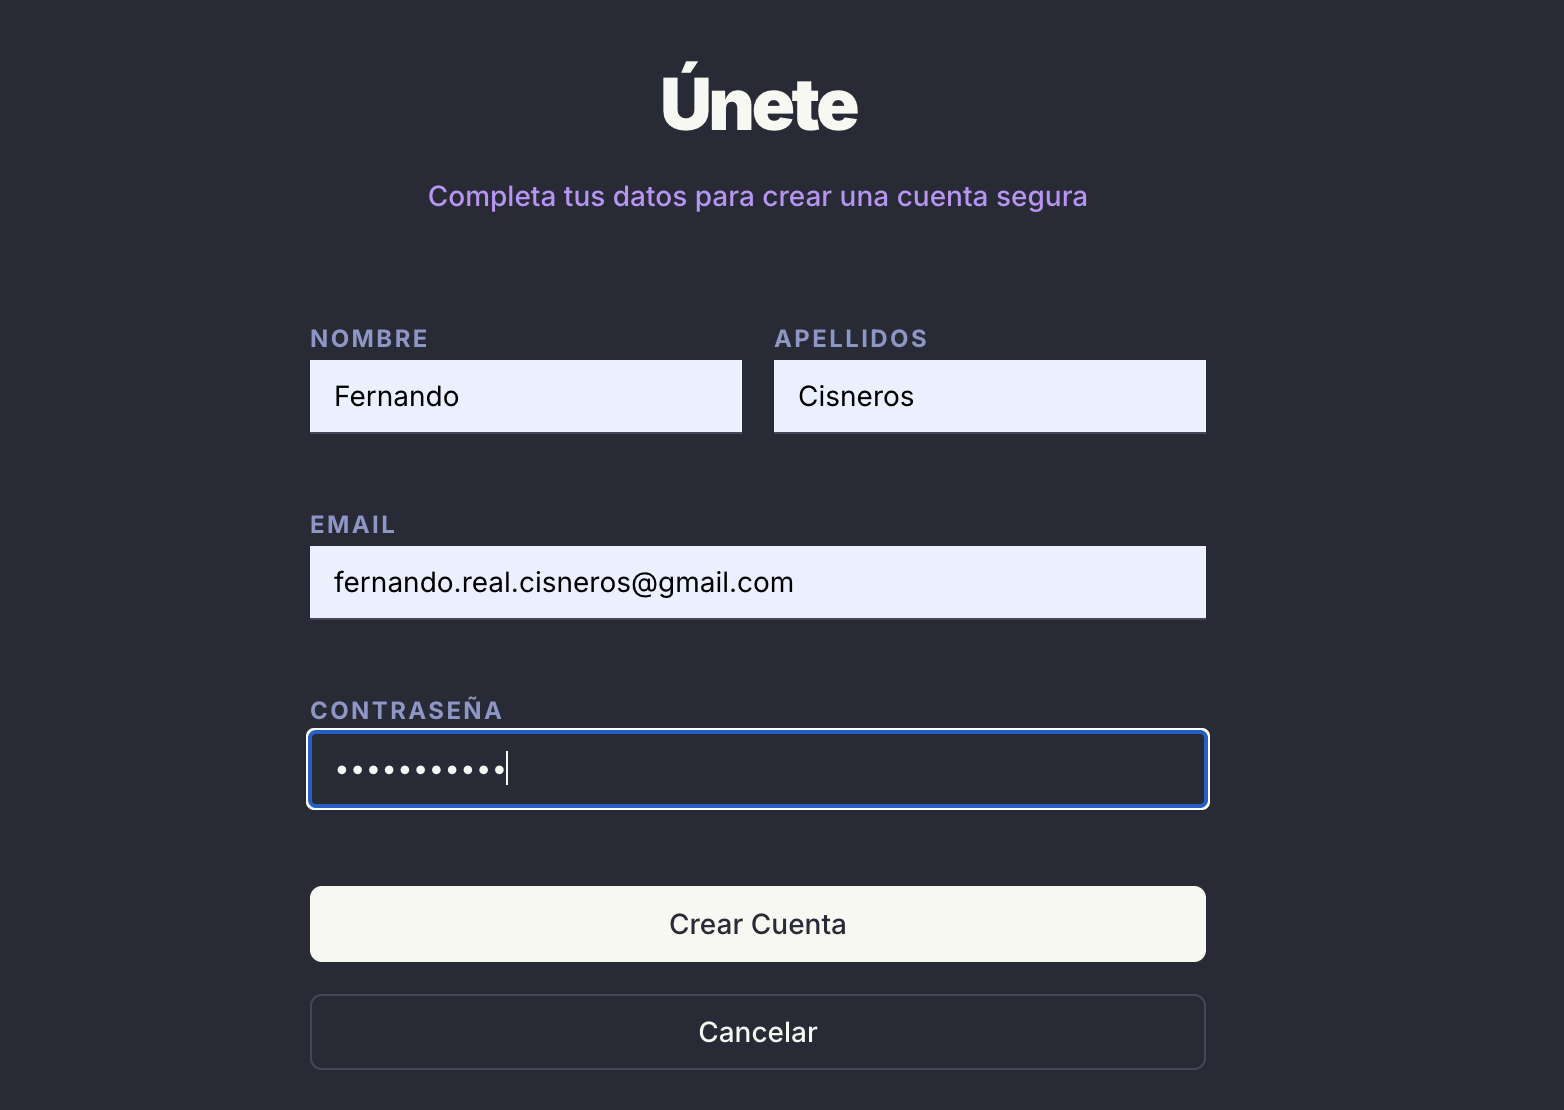
\includegraphics[width=0.6\textwidth]{imagenes/02_usuario/03_creacionDeUsuario.png}
    \caption{Formulario de registro de usuario.}
\end{figure}

El formulario requiere rellenar los siguientes campos:
\begin{itemize}
    \item \textbf{Nombre:} Nombre de pila del usuario.
    \item \textbf{Apellidos:} Apellidos del usuario.
    \item \textbf{Correo electrónico:} Dirección válida que servirá como identificador único y medio para verificar la cuenta.
    \item \textbf{Contraseña:} Credencial secreta. Debe cumplir con criterios mínimos de seguridad.
    \item \textbf{Confirmación de contraseña:} Para asegurar que no hay errores tipográficos.
\end{itemize}

\begin{figure}[!ht]
    \centering
    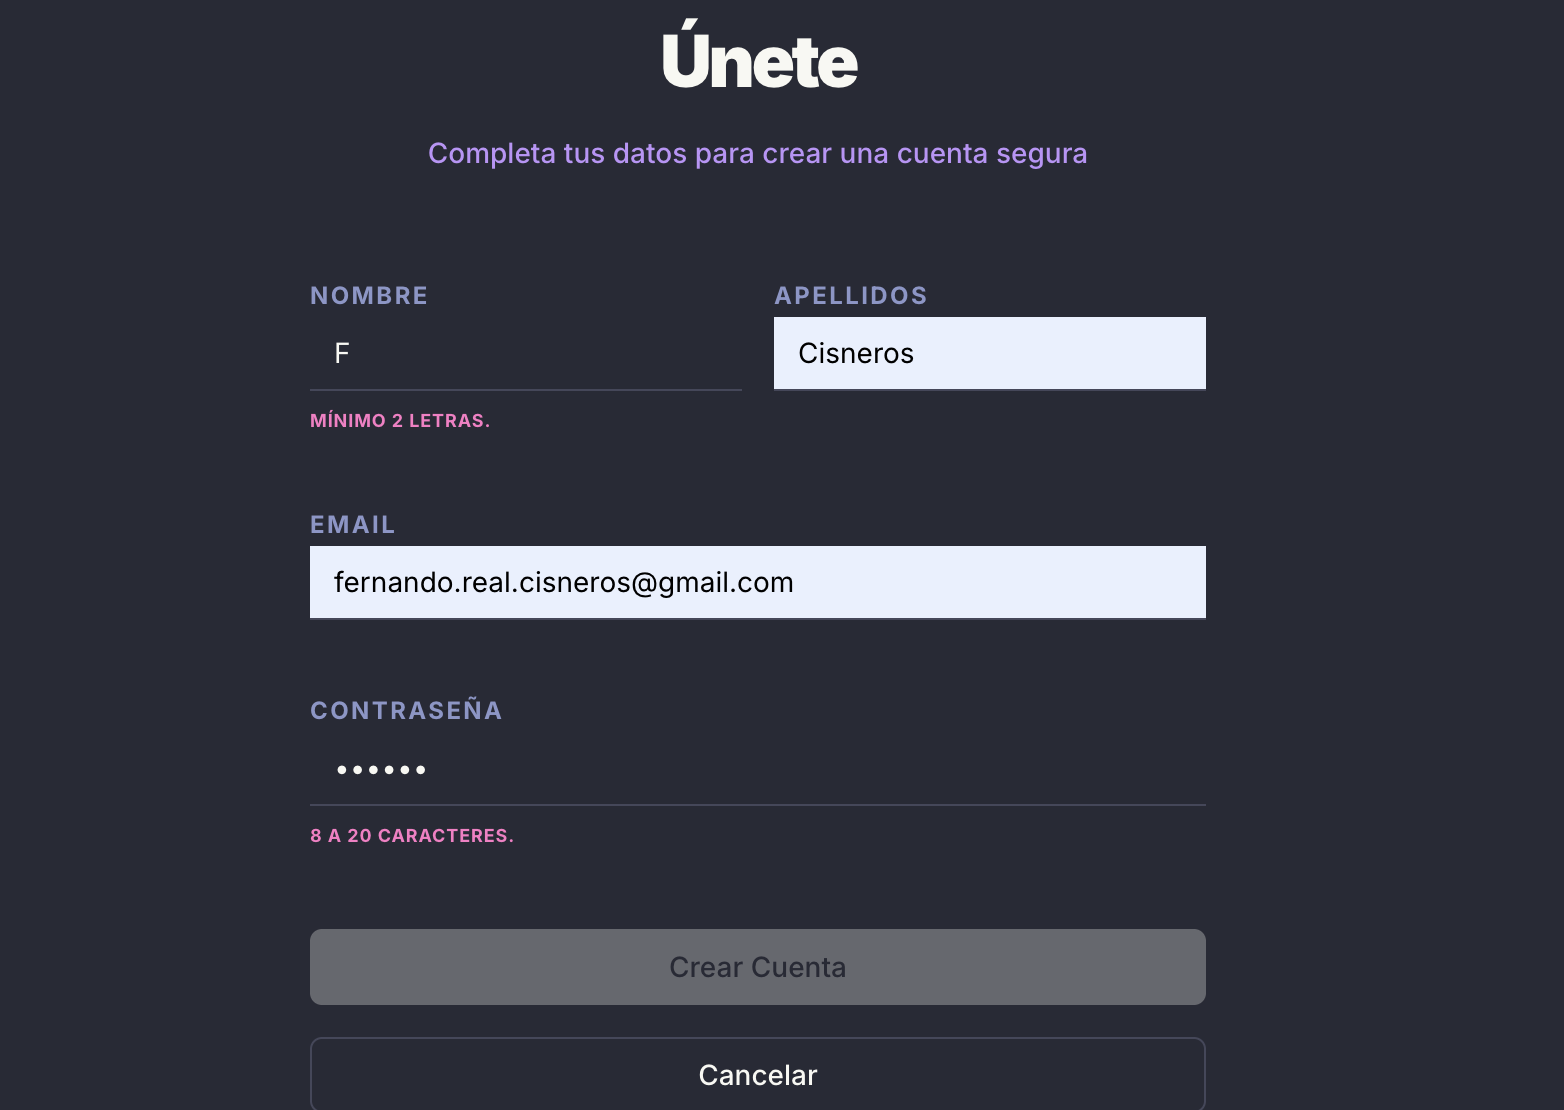
\includegraphics[width=0.6\textwidth]{imagenes/02_usuario/02_validacionRegistroNuevoUsuario.png}
    \caption{Validación de campos en el formulario de registro.}
\end{figure}

Si los datos introducidos no cumplen los requisitos (por ejemplo, correos electrónicos mal formateados o contraseñas que no coinciden), la aplicación mostrará alertas de validación, impidiendo el registro hasta que se corrijan los errores.

\begin{figure}[!ht]
    \centering
    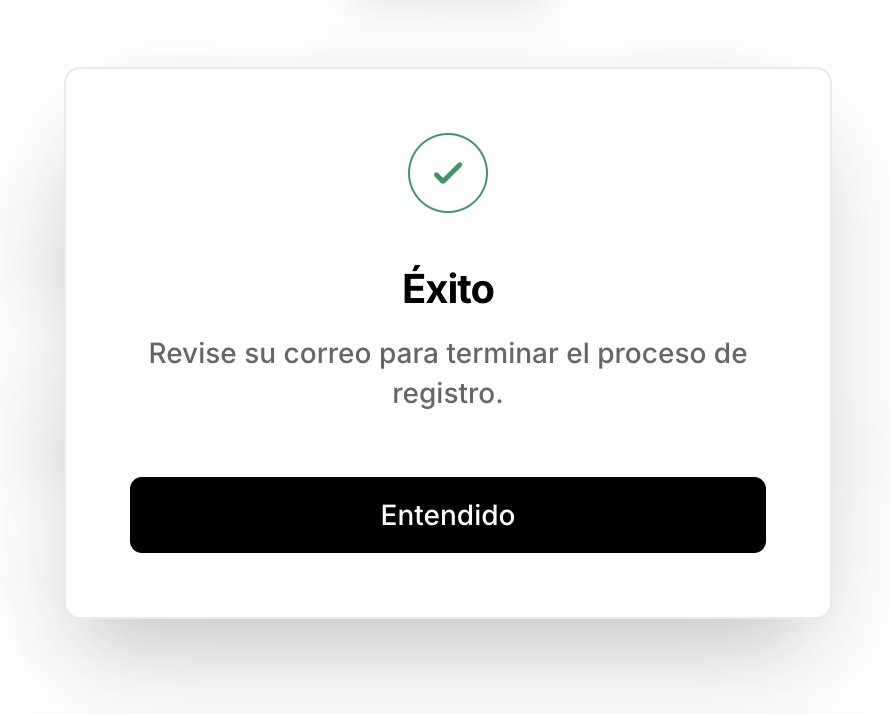
\includegraphics[width=0.6\textwidth]{imagenes/02_usuario/04_CreacionConExitoDeNuevoUsuario.png}
    \caption{Mensaje de éxito tras el registro y aviso de verificación de correo.}
\end{figure}

Tras enviar el formulario correctamente, la aplicación notifica que la cuenta ha sido creada y que es imperativo verificar la dirección de correo electrónico antes de poder iniciar sesión por primera vez.

\subsection{Verificación de Correo Electrónico}

En entornos de desarrollo y pruebas, el sistema captura los correos electrónicos enviados a través de una herramienta integrada (\textit{MailHog}).

\begin{figure}[!ht]
    \centering
    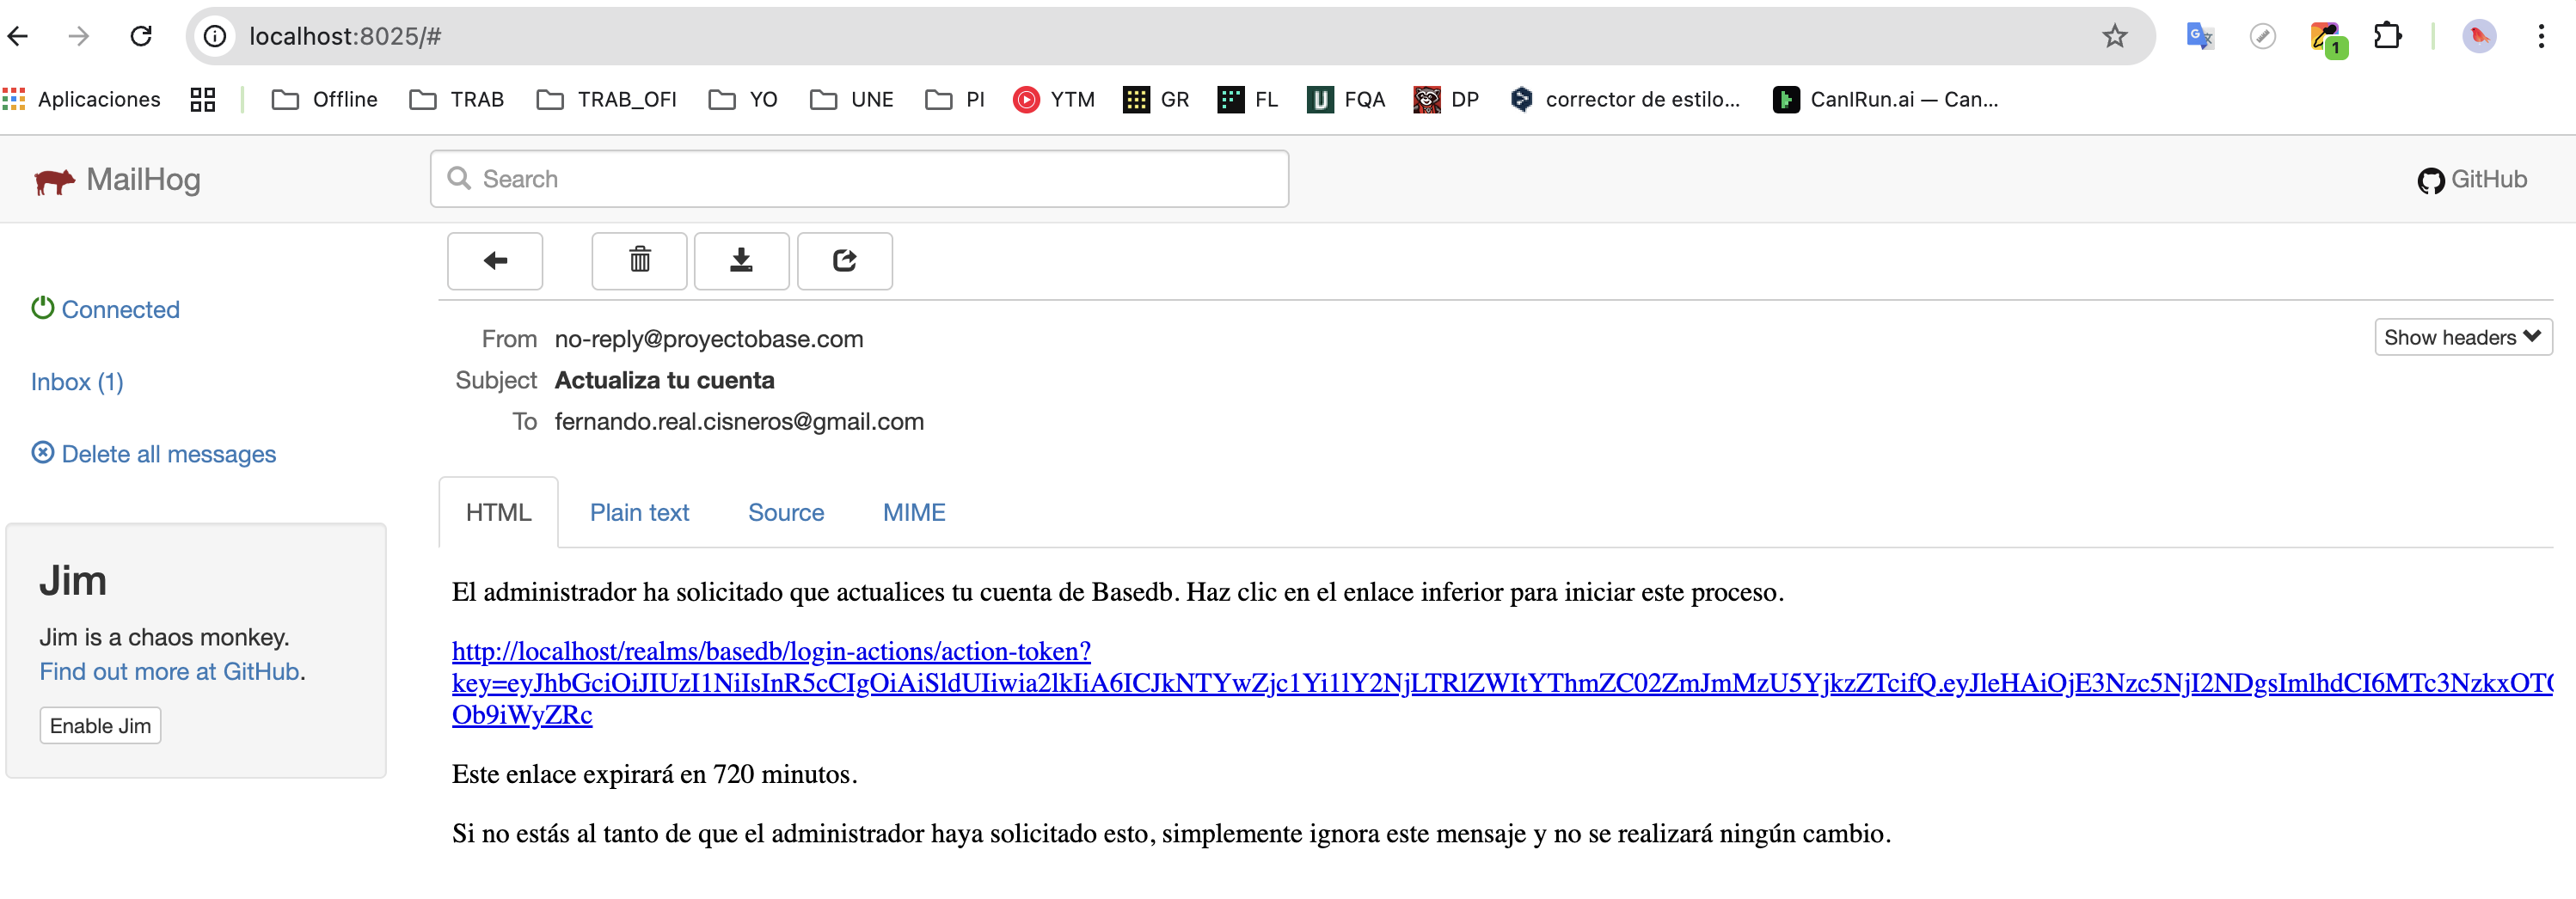
\includegraphics[width=\textwidth]{imagenes/02_usuario/05_verificarMailConElEntornoDeDesarrolloMailHog.png}
    \caption{Buzón de correo simulado para verificar la cuenta.}
\end{figure}

\begin{figure}[!ht]
    \centering
    
\includegraphics[width=0.6\textwidth]{imagenes/02_usuario/06_linkDeVerificarEnKeyCloak.png}
    \caption{Enlace de verificación de correo electrónico.}
\end{figure}

Al abrir el correo recibido, el usuario debe pulsar el enlace proporcionado para confirmar que es el propietario de la dirección indicada. Este paso interactúa directamente con el sistema de seguridad subyacente.

\begin{figure}[!ht]
    \centering
    
\includegraphics[width=0.6\textwidth]{imagenes/02_usuario/07_linkDeVolverAAplicacion.png}
    \caption{Confirmación de correo electrónico verificado.}
\end{figure}

\begin{figure}[!ht]
    \centering
    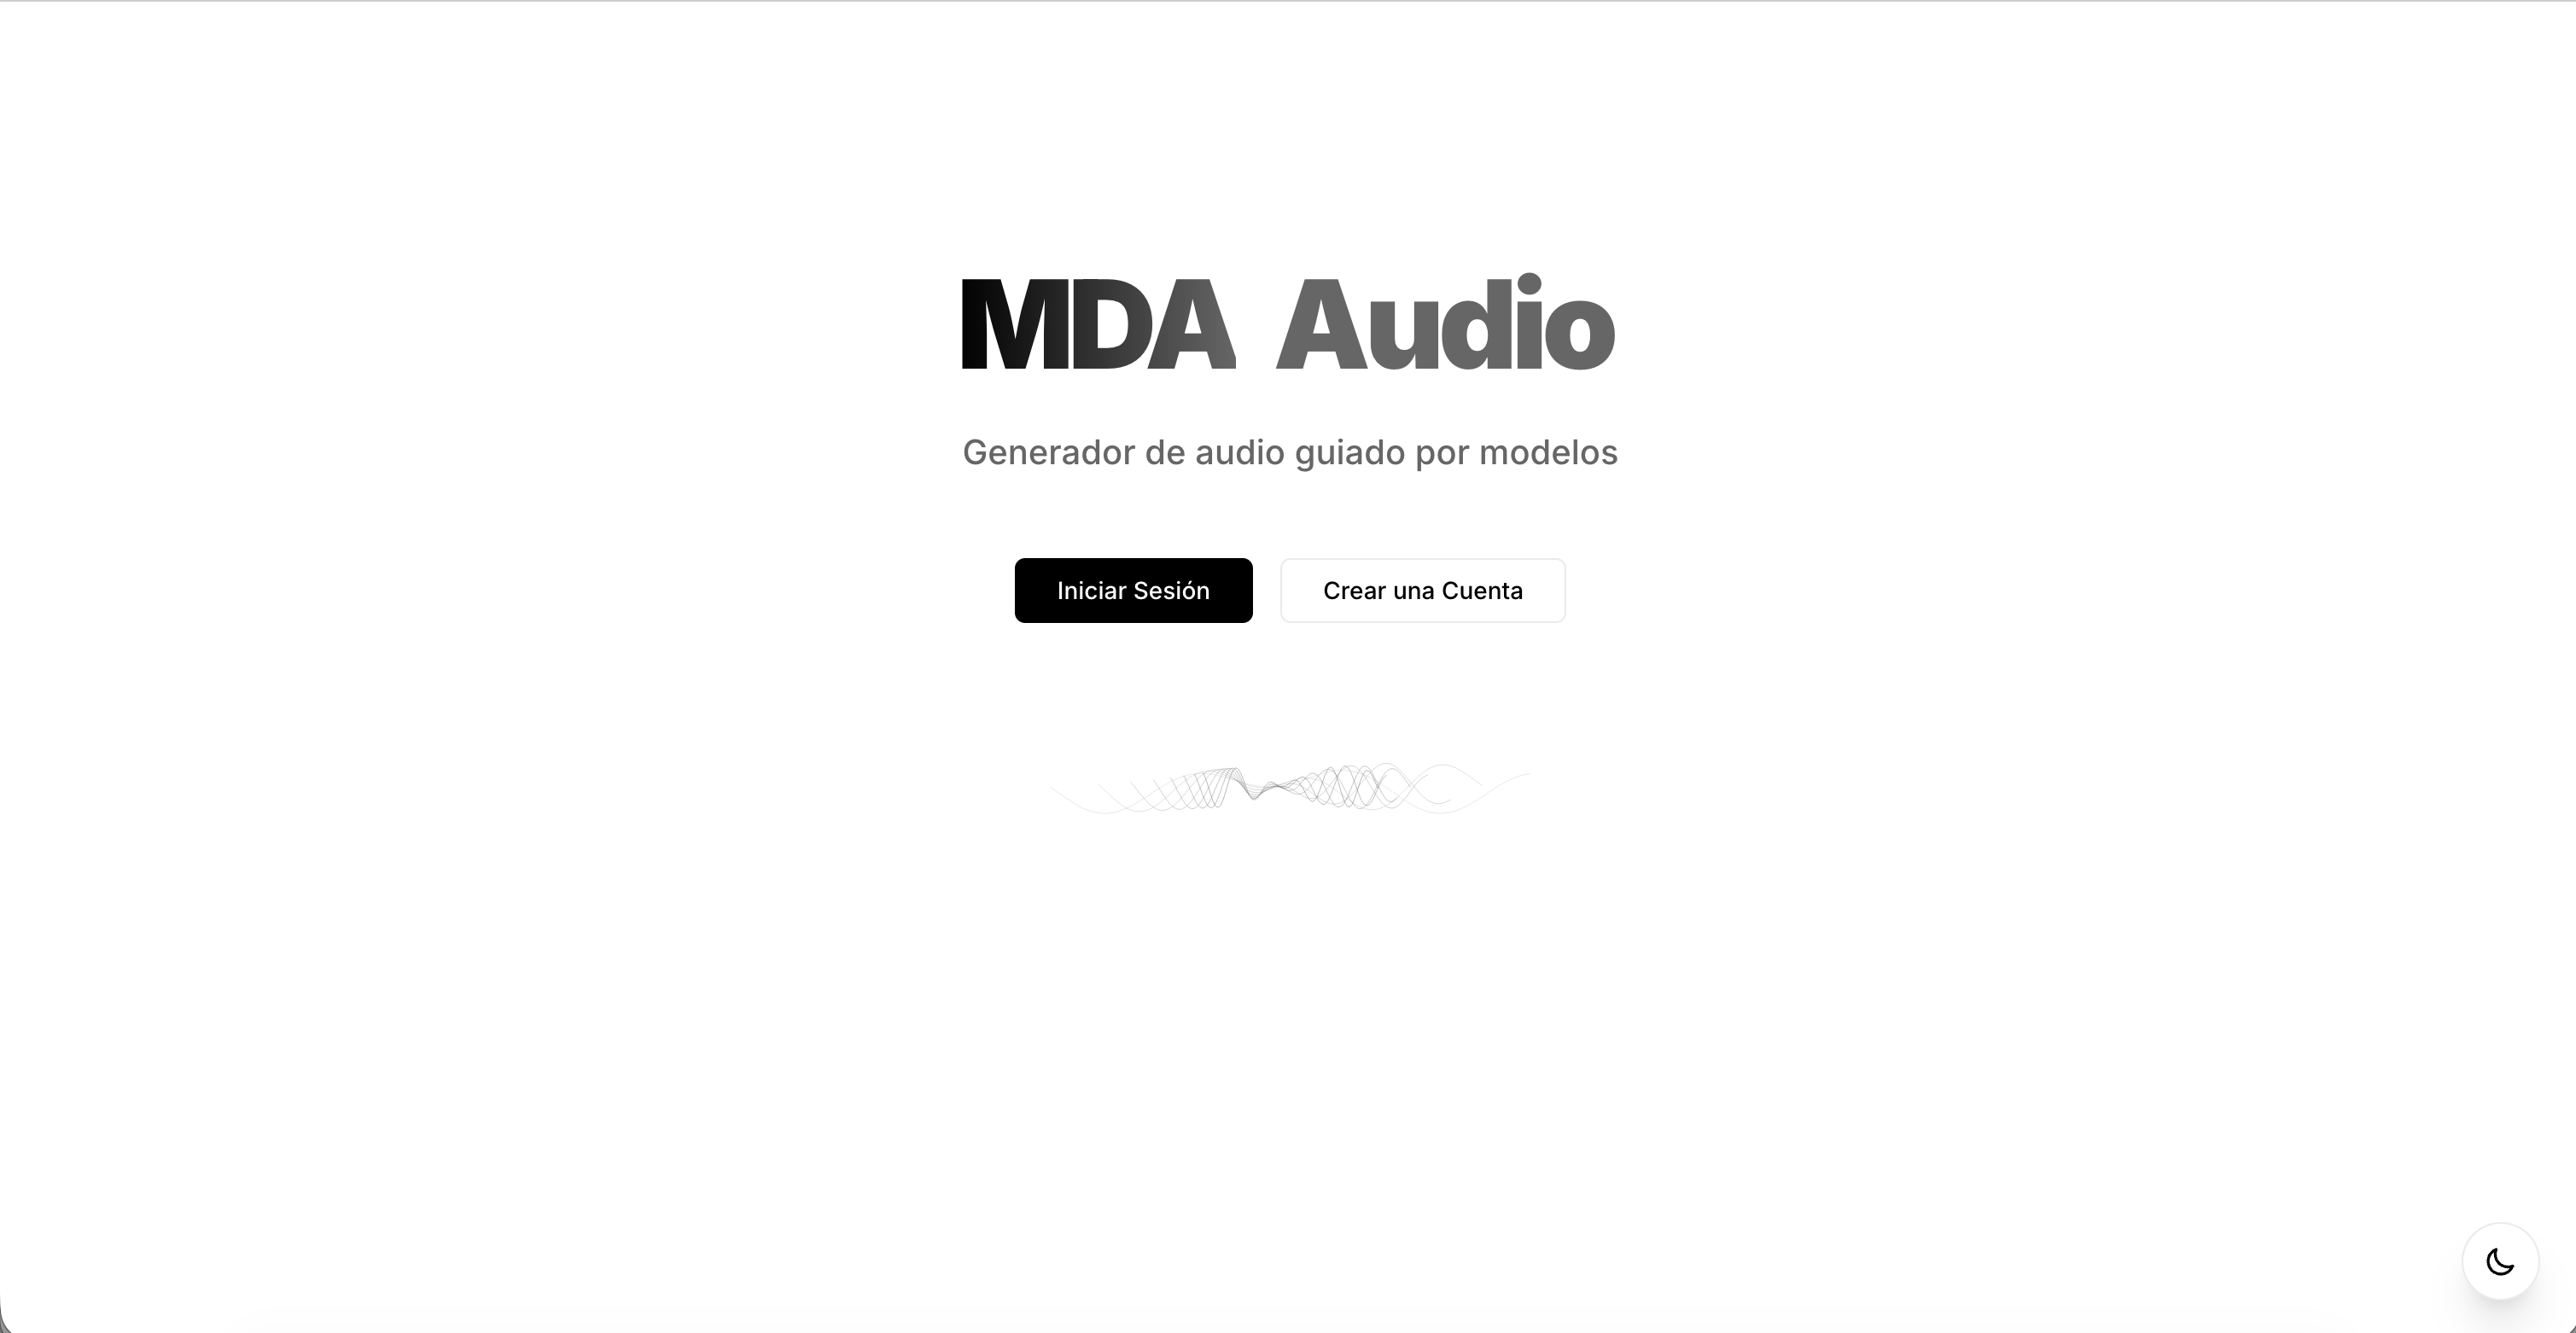
\includegraphics[width=0.6\textwidth]{imagenes/02_usuario/09_volverAAplicacion.png}
    \caption{Enlace para volver a la aplicación tras la verificación.}
\end{figure}

Una vez verificada la cuenta, se mostrará un mensaje de confirmación y un enlace directo para regresar a la aplicación \textit{MDAA} y proceder al inicio de sesión.

\subsection{Inicio de Sesión y Acceso}

Con la cuenta verificada, el usuario ya puede autenticarse.

\begin{figure}[!ht]
    \centering
    
\includegraphics[width=0.5\textwidth]{imagenes/02_usuario/10_botonInicioSesion.png}
    \caption{Botón de inicio de sesión.}
\end{figure}

Al pulsar el botón de iniciar sesión desde la pantalla principal, se redirige al usuario a la pasarela segura.

\begin{figure}[!ht]
    \centering
    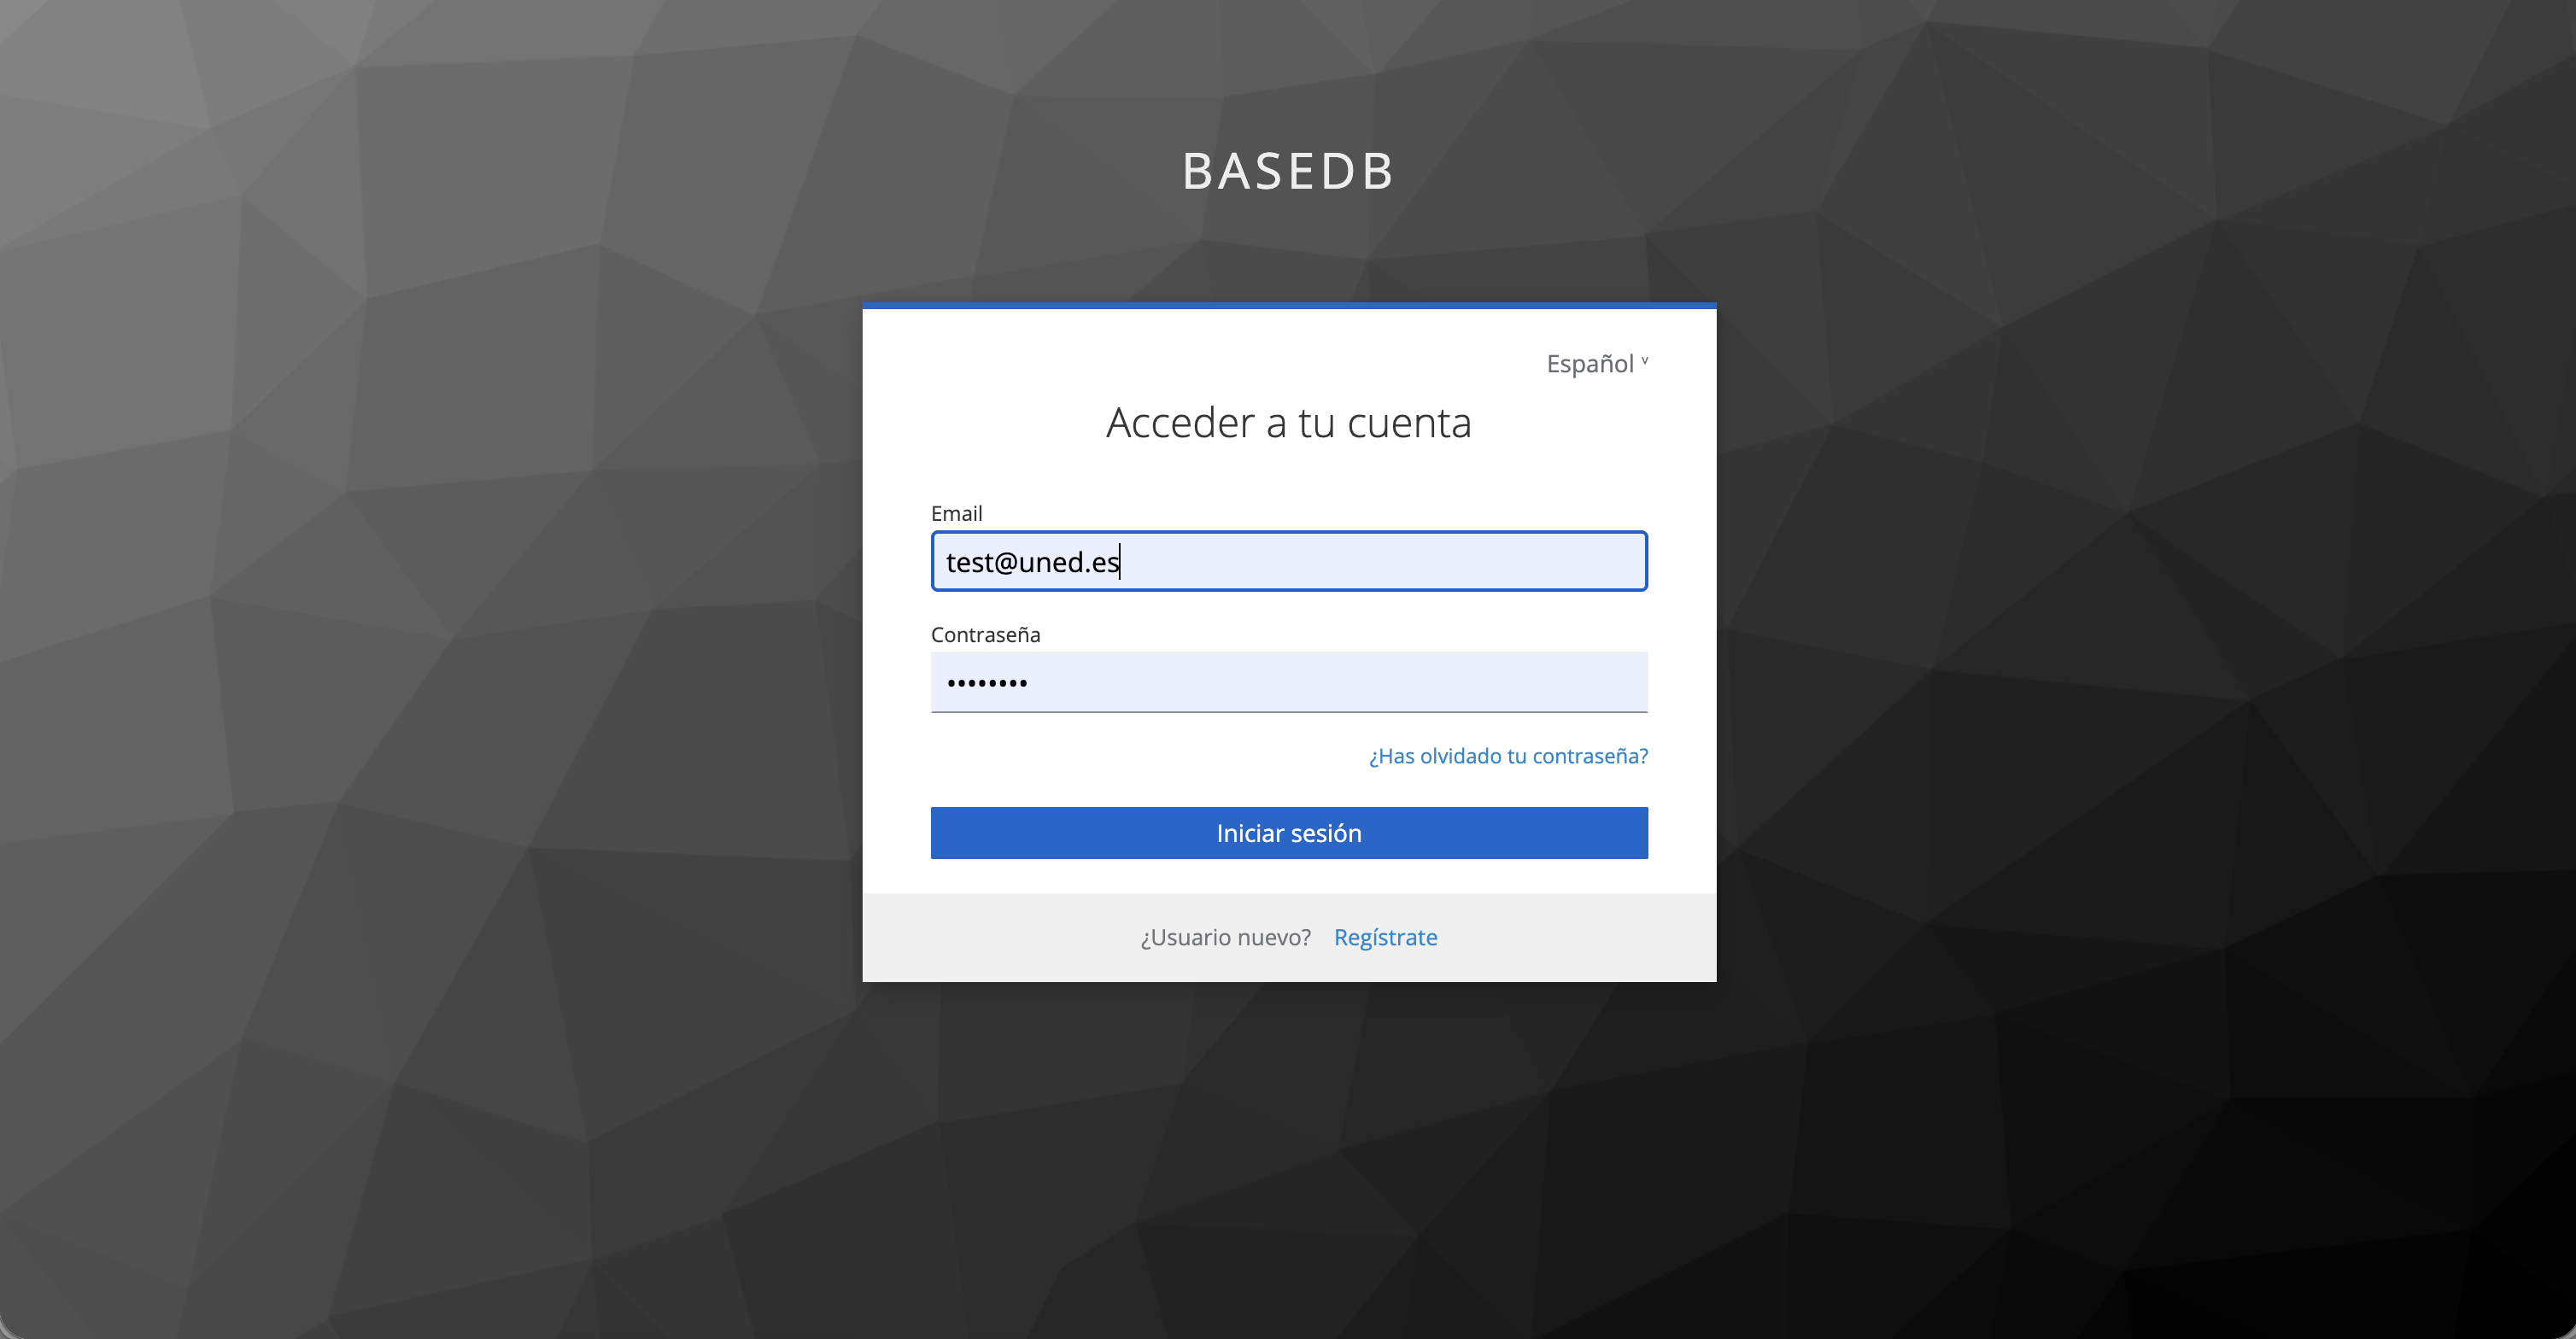
\includegraphics[width=0.6\textwidth]{imagenes/02_usuario/11_loginConUsarioTestQueDebemosUtilizarParaProbar.png}
    \caption{Formulario de inicio de sesión con usuario de pruebas.}
\end{figure}

En este formulario, se deben introducir:
\begin{itemize}
    \item \textbf{Usuario o correo electrónico:} Identificador registrado. Para pruebas se puede utilizar un usuario preconfigurado (\textit{test}).
    \item \textbf{Contraseña:} La clave asociada a la cuenta.
    \item \textbf{Opciones adicionales:} Enlaces para recuperar contraseñas olvidadas si estuviesen configuradas.
\end{itemize}

\begin{figure}[!ht]
    \centering
    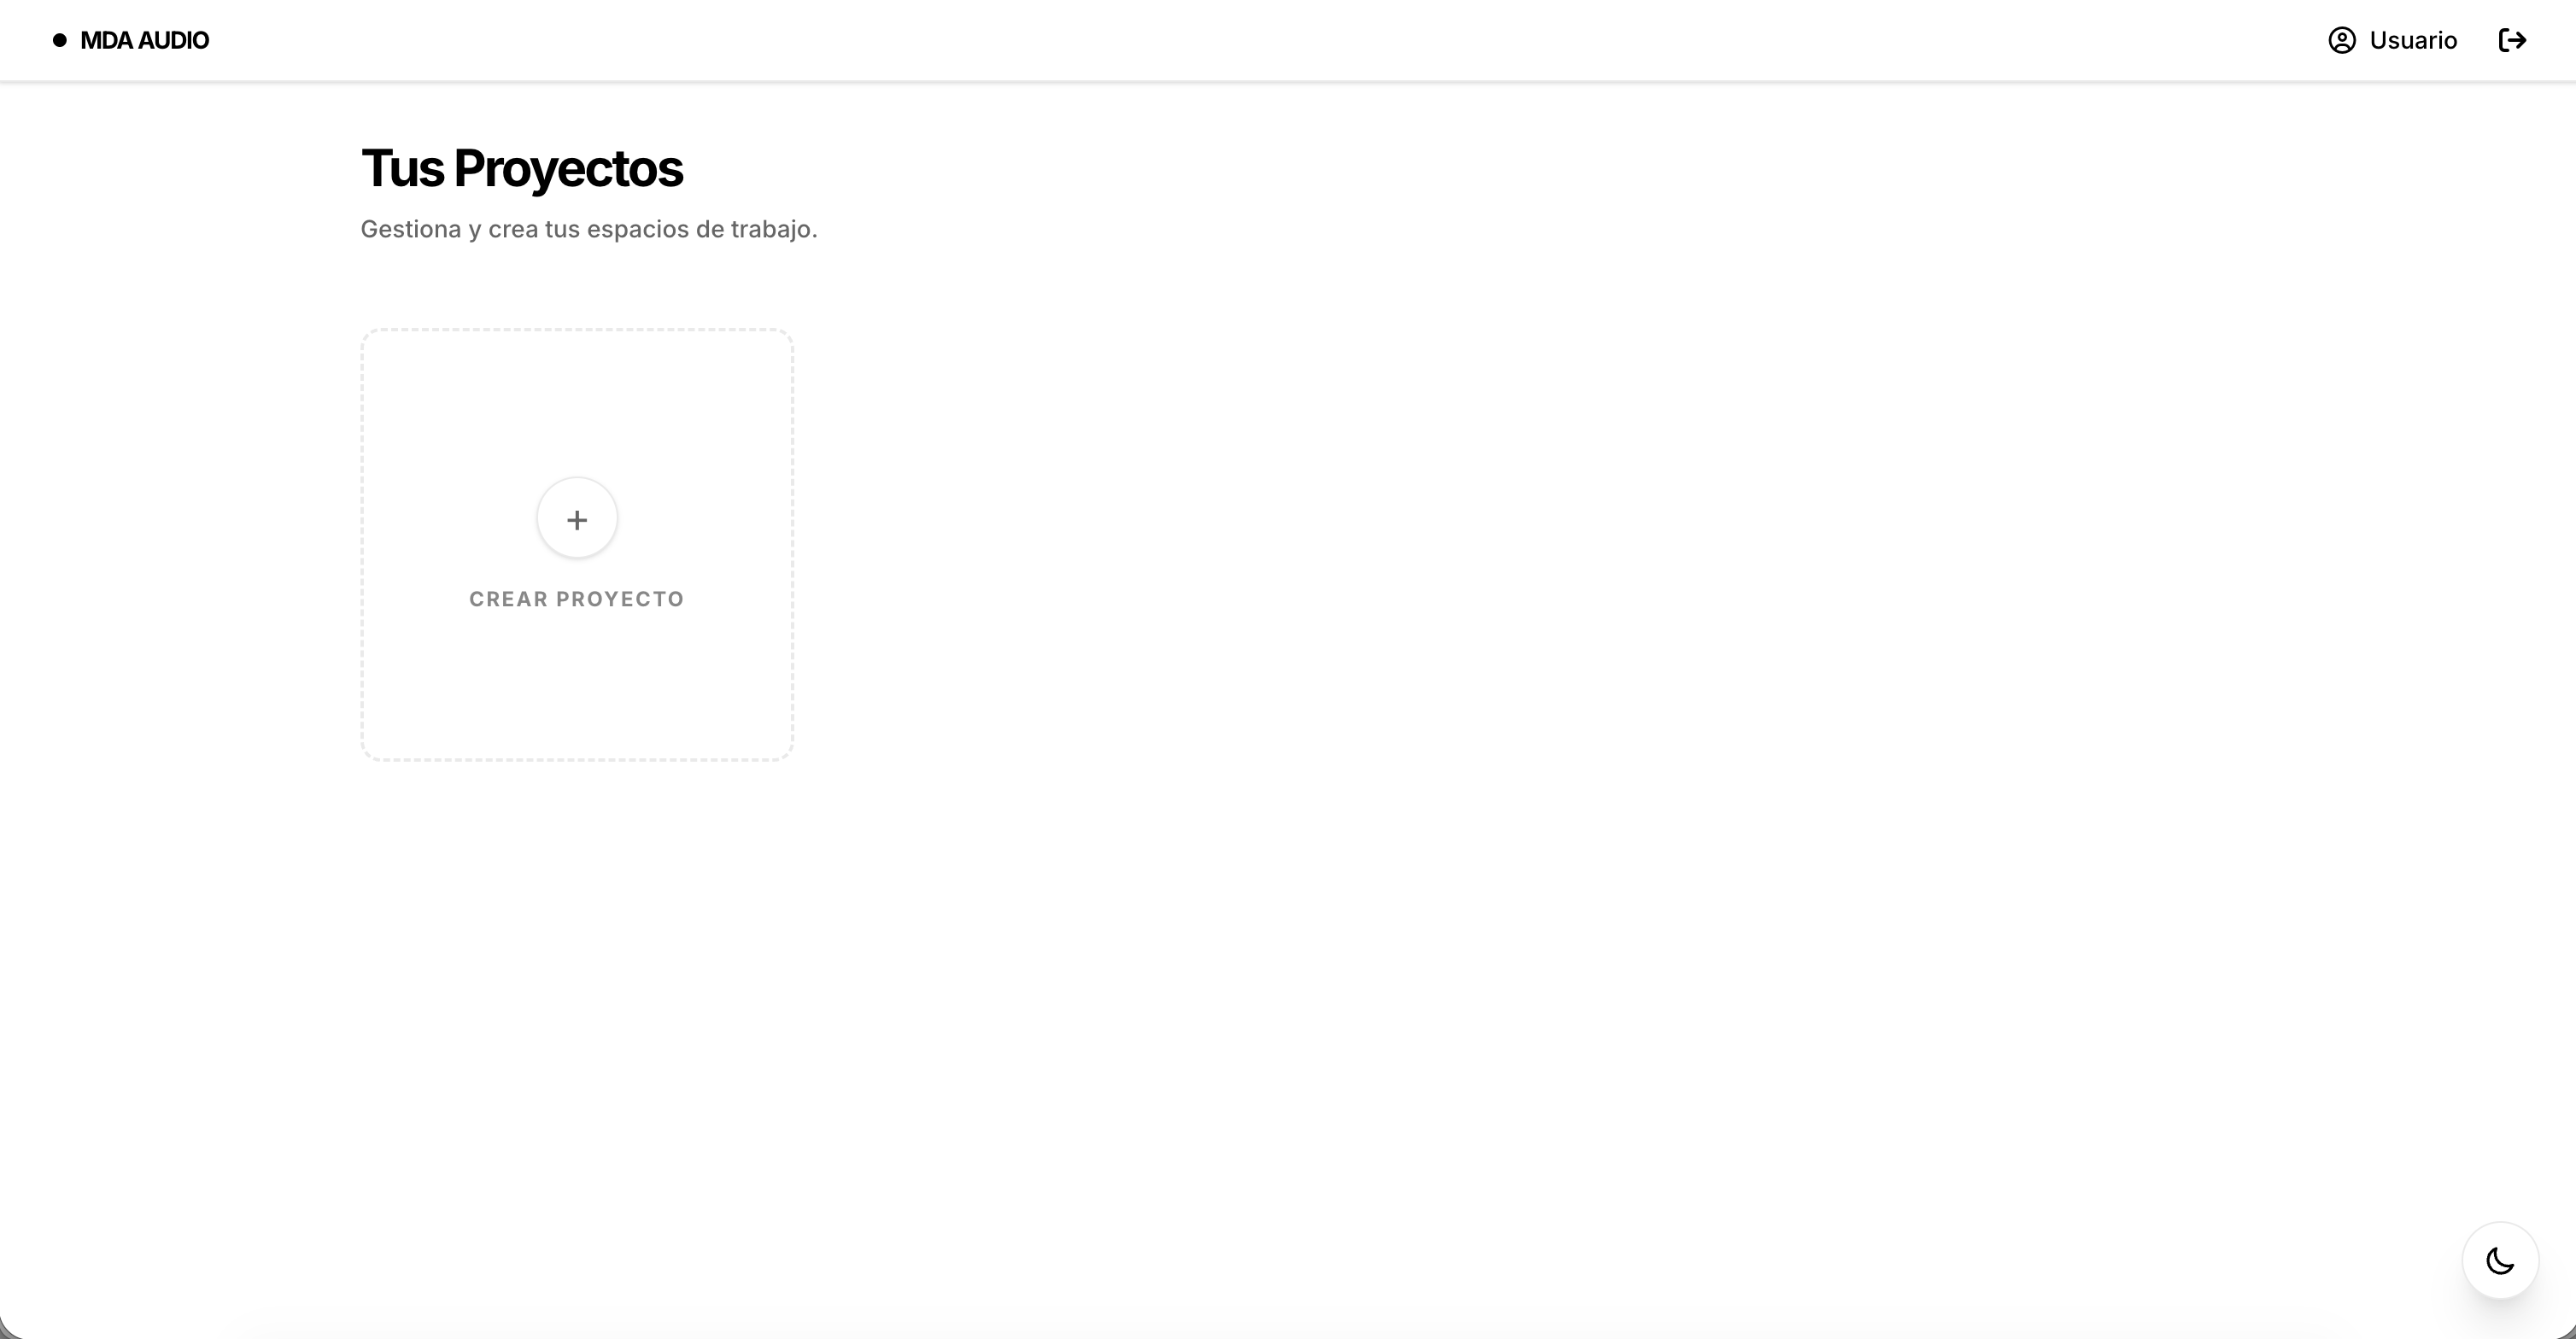
\includegraphics[width=\textwidth]{imagenes/02_usuario/12_entradaEnLaAplicacion.png}
    \caption{Pantalla principal tras iniciar sesión exitosamente.}
\end{figure}

Si las credenciales son correctas, el sistema autentica al usuario y le redirige a su área de trabajo personal, donde se listan sus proyectos y se habilita la interacción con los módulos de generación de código y validación \textit{DSL}.
